\section{Implementation}

Our task is to do \textit{IoT data analytics with serverless computing}, therefore as a first step
we started out by thinking about the underlying infrastructure. We decided on using Apache Kafka for
streaming, \textit{MongoDB} as our database and \textit{OpenFaaS} as the serverless platform.

The decision to use \textit{OpenFaaS} was made because of its ease to deploy a stack of services
using \textit{Docker Swarm}. While doing research we came across many different serverless
frameworks. \textit{OpenWhisk}, \textit{Fission} and \textit{Kubeless} just to name a few. While all
of those seem to have their benefits, none of them seemed to be as versatile as \textit{OpenFaaS}.
\textit{OpenFaaS} poses itself to have first class support for \textit{Docker Swarm} and being
\textit{Kubernetes} native. The former was particularly interesting for us as this meant that we
could test the framework without having to install any external tool except for  \textit{Docker}.
Running was as simple as cloning the \textit{OpenFaaS} repository, calling \texttt{docker swarm
init} and executing the provided initialisation script. Deploying an actual function is equally as
simple. One has the option to either deploy a function from the store through the nicely designed
\textit{OpenFaaS} gateway on port 8080 or with the preferred way, which is using the
\texttt{faas-cli}. Deploying a function from the store with it would look as follows

\begin{lstlisting}[language=bash]
$ faas store deploy figlet
\end{lstlisting}

where \texttt{figlet} is the name of the function in the store.

After gaining a grasp of how the platform works, we decided to put our own spin on it by firstly
modifying the given deploy script to our needs and porting it from \textit{Bash} to \textit{Rust}
for it to be cross platform. The next step then was to write our own configuration file for swarm
deployment, namely \texttt{deploy.yml}. This \textit{YAML} file includes the configuration for
\textit{Kafka}, \textit{Zookeeper}, \textit{MongoDB}, various services that are needed for
\textit{OpenFaaS}, a bunch of gateways for visualisation and the \textit{Kafka-Connector}. The
latter is particularly interesting, because its main purpose is to call a serverless function on a
Kafka topic change. To make a function react to a Kafka topic we can again use our example store
function \texttt{figlet}

\begin{lstlisting}[language=bash]
$ faas store deploy figlet --annotation topic="faas-request"
\end{lstlisting}

The deployment aspect is the same as before therefore the interesting part is the
\texttt{--annotation} flag, where \texttt{topic="faas-request"} is the \textit{Kafka} topic the
function is supposed to listen to and act on. We subsequently can look for the result in the logs of
the connector service.

While our technology stack for the most part was nice to work with, we still had our fair share of
problems. The most significant so far was in relation to our \textit{MongoDB} database.
\textit{MongoDB}'s API design is confusing to say the least. Questionable deprecation choices and
multiple connect interfaces are the most rampant examples. Unfortunately those were not the only
problems in that regard we ran into. Connecting through a node instance natively on the system would
work fine, however connecting through a deployed function in \textit{OpenFaaS} was not possible.
After applying various fixes the function was finally able to connect.

The next challenge will be to post to the database through the \textit{Kafka-Connector}. When that
is done we can finally focus on gathering data from IoT devices.

\newpage

\subsection{Functions}

With the OpenFaaS framework, every function consists of three parts: a function template, the
function's source code and a definition file.

Function templates are categorised by the programming language the corresponding function is written
in. At the bare minimum, a template contains a \texttt{Dockerfile} and a \texttt{template.yml}. The
\texttt{Dockerfile} has to be written in a way such that a \texttt{function} directory on the same
directory level is copied into the image. During the build step, this \texttt{function} directory
contains the source code, so depending on the programming language, it either has to be compiled or
moved to the correct location straight away. Additionally, the \texttt{Dockerfile} has to install
the \textit{OpenFaaS Watchdog}. The \textit{OpenFaaS Watchdog} is a service which is used to connect
the function to the \textit{OpenFaaS} gateway. Historically, the watchdog would pass requests to the
function via \textit{Standard Input} and the return the function's \textit{Standard Output} as the
response. With this method however, the function could not control any aspect of the \textit{HTTP}
request and response. The new version of the \textit{OpenFaaS Watchdog} offers a few more operation
modes. The first, called \texttt{http}, forwards the received request to a specified port in the
function. This means that function templates using this mode have to be written in such a way that
they include an web server. This way the function can consume the \textit{HTTP} request directly,
which also makes calling functions easier since they can use standard \textit{HTTP} methods and
status codes. Another new mode is \texttt{static}, which can be used to create very simple functions
serving static files. \cite{of-watchdog} The \texttt{template.yml} file contains the metadata for
the function. This file can be empty, i.e. all metadata is optional, but most commonly it contains
at least the \texttt{language} property used to specify the programming language the template is
meant for. \cite{openfaas-build-functions} Commonly, a \texttt{function} directory containing a
“Hello, world!” function is included in the template itself to serve as a starting point when
creating a new function from scratch.

Another part needed for building a function is a definition file containing the name of the function
and all other data needed to deploy the functions. One essential part of this definition file is the
gateway URL, which the \textit{OpenFaaS Watchdog} uses to connect to the \textit{OpenFaaS} gateway.

\begin{figure}[H]
  \begin{lstlisting}
version: 1.0
provider:
  name: openfaas
  gateway: http://127.0.0.1:8080
functions:
  filter:
    lang: rust-http
    handler: ./filter
    image: filter:latest
    environment:
      RUST_LOG: info
      write_debug: 'true'
      gateway_url: http://gateway:8080
  \end{lstlisting}
  \caption{A definition file for a Rust function called \texttt{filter}.}
  \label{fig:function-definition}
\end{figure}

In \autoref{fig:function-definition} we can see that there are two different gateway URLs. The
first one, \texttt{provider.gateway}, is used by the \texttt{faas-cli} command line tool in order to
know where to deploy the function to. The second one,
\texttt{functions.filter.environment.gateway\_url} is the URL the gateway can be reached from inside
the cluster and the one passed to the \textit{OpenFaaS Watchdog}. Furthermore, the function template
is specified using \texttt{functions.filter.lang}, the path the the function's source code is given
by \texttt{functions.filter.handler} and the name of the \textit{Docker} image is specified by
\texttt{functions.filter.image}.

Assuming the definition file shown in \autoref{fig:function-definition} is called
\texttt{filter.yml}, we can build the function using the following command:

\begin{lstlisting}[language=bash]
faas-cli build -f filter.yml
\end{lstlisting}

Once built, the function can be deployed using an equally simple command:

\begin{lstlisting}[language=bash]
faas-cli deploy -f filter.yml
\end{lstlisting}

\subsection{Mobile Application}

Another one of our tasks was to create a mobile application that fetches data from the respective
device and sends data to a \textit{Kafka} topic which subsequently invokes a \textit{serverless
function} to finally persist that data in a \textit{MongoDB} database. To approach this topic we
first did some research on current possibilities on creating cross platform mobile applications and
the general feasibility of the task at hand. It became quite apparent early on that the desired
design for the application is not possible on \textit{iOS}.

The idea for the design of the app is actually rather simple. Get data from the device, no matter if
the application is in foreground, background or the screen is off and the device subsequently
basically being in standby. On \textit{Android} this can be realised easily with a so called
\textit{ForegroundService}. On \textit{iOS} going for the same approach is difficult because of its
restrictions on background tasks. While obviously applications like music players can run in the
background on that platform, achieving the same for a highly battery intensive app like the one we
are developing, is more or less impossible.

Mainly for that reason we actually chose to go for a cross platform mobile application, so we can
have a fully supported \textit{Android} version and also an \textit{iOS} version with limited
functionality.

Finding the ideal tool for our job of creating an application supporting both \textit{iOS} and
\textit{Android} seemed at first pretty easy. We chose to use \textit{React Native} as we both
already have experience with \textit{React} itself and the approach to \textit{UI design} seemed
equally elegant.

Getting started with \textit{React Native} was rather fast and effortless, the same however could
not be said anymore once we progressed further with the project. At first things were looking good
as the UI did properly respond to data from sensors / CPU but as we added more and more data for
display, the UI got more and more sluggish to the point that it could not be considered usable
anymore. Unfortunately this was not the only problem.

By nature the application relies heavily on \textit{native code}. The main culprit for this is the
\textit{ForegroundService} on \textit{Android}. \textit{React Native} has a so called
\textit{bridge} for communication between \textit{native code} and the \textit{UI}. Our application
uses that bridge heavily for retrieving information from the service and also to push data to the
service.

Once we fully implemented the settings view and were basically finished with the application, the
app started to crash constantly on \textit{Android}. Unfortunately the tooling of \textit{React
Native} really does not help with debugging fatal crashes. So we had to make a conscious decision
whether we want to continue with \textit{React Native} or start over with something else entirely.

In the end we concluded to search for other frameworks as we deemed \textit{React Native} as
incompatible for our task. We then decided on using \textit{Flutter}. \textit{Flutter} is a modern
cross platform mobile application framework by \textit{Google}. \textit{Flutter} compiles down to
native code and therefore should have a performance advantage compared to \textit{React Native}.

As with any new programming language, \textit{Dart} - the language behind \textit{Flutter} - took
some time to get used to and be productive with. After a while however the process of designing
\textit{UIs} with \textit{Flutter} and writing logic was rather seamless. Fortunately the native
part of the \textit{React Native} application could almost fully be reused for the \textit{Flutter}
version of the app. The surprisingly easy to use \textit{bridge} between native code and
\textit{Dart} in \textit{Flutter} made the transition from \textit{React Native} regarding native
code on \textit{Android} painless.

One of the reason we first chose to use \textit{React Native} was the extensive community support.
Getting sensor data from almost all supported sensors on \textit{iOS} was as simple as including a
package. The same cannot be said about \textit{Flutter}. For that reason we also had to write some
native code for \textit{iOS} which splits the code base further.

The finished application now contains four Views:

\begin{figure}[H]
  \centering
  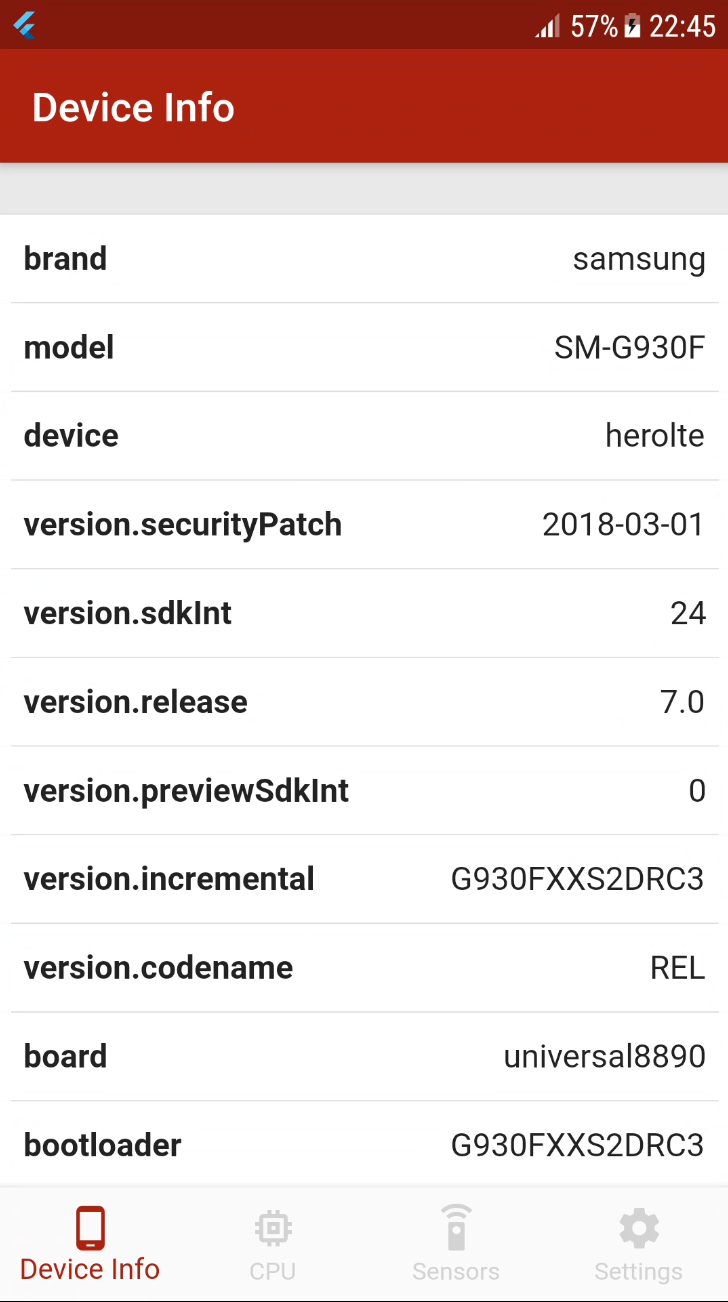
\includegraphics[height=20em]{mobile-device-info}
  \caption{\textit{Device Info} contains various information about the running system.}
\end{figure}

\begin{figure}[H]
  \centering
  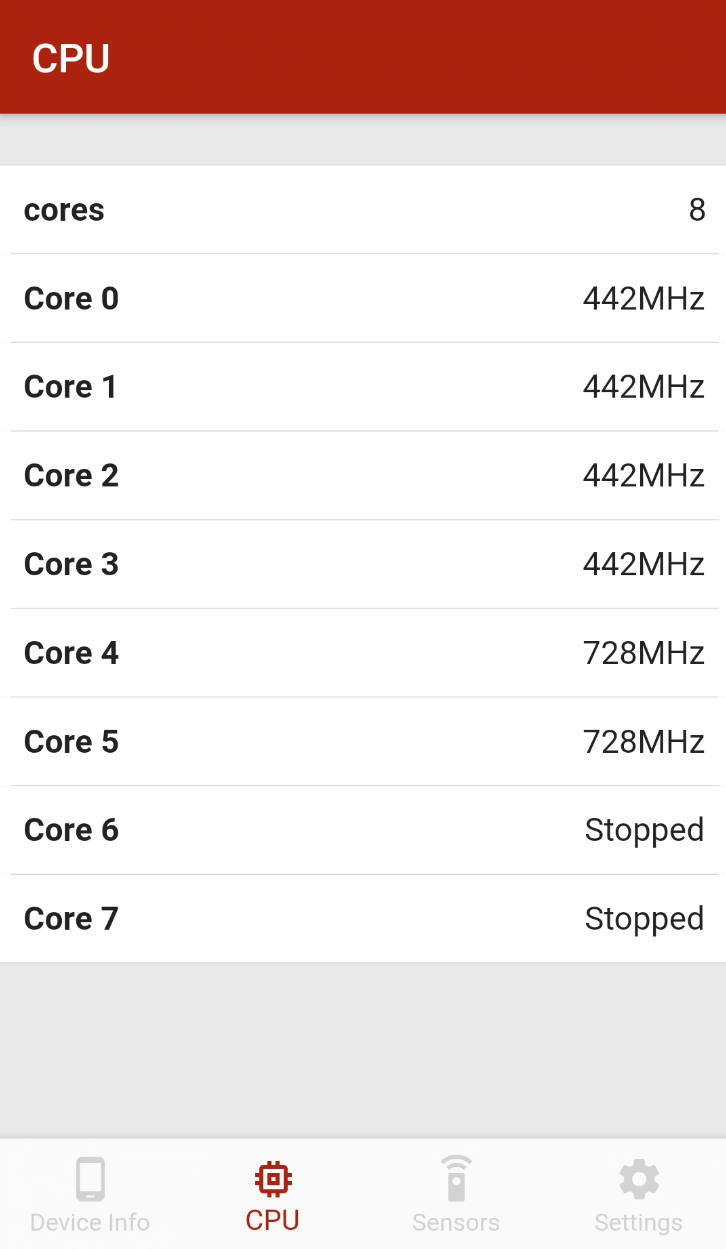
\includegraphics[height=20em]{mobile-cpu}
  \caption{\textit{CPU} shows the amount of cores available and the frequency they are currently
  running at, if they are running at all. This view, however, is only available on \textit{Android}
  due to limitations on retrieval of CPU information on \textit{iOS}.}
\end{figure}

\begin{figure}[H]
  \centering
  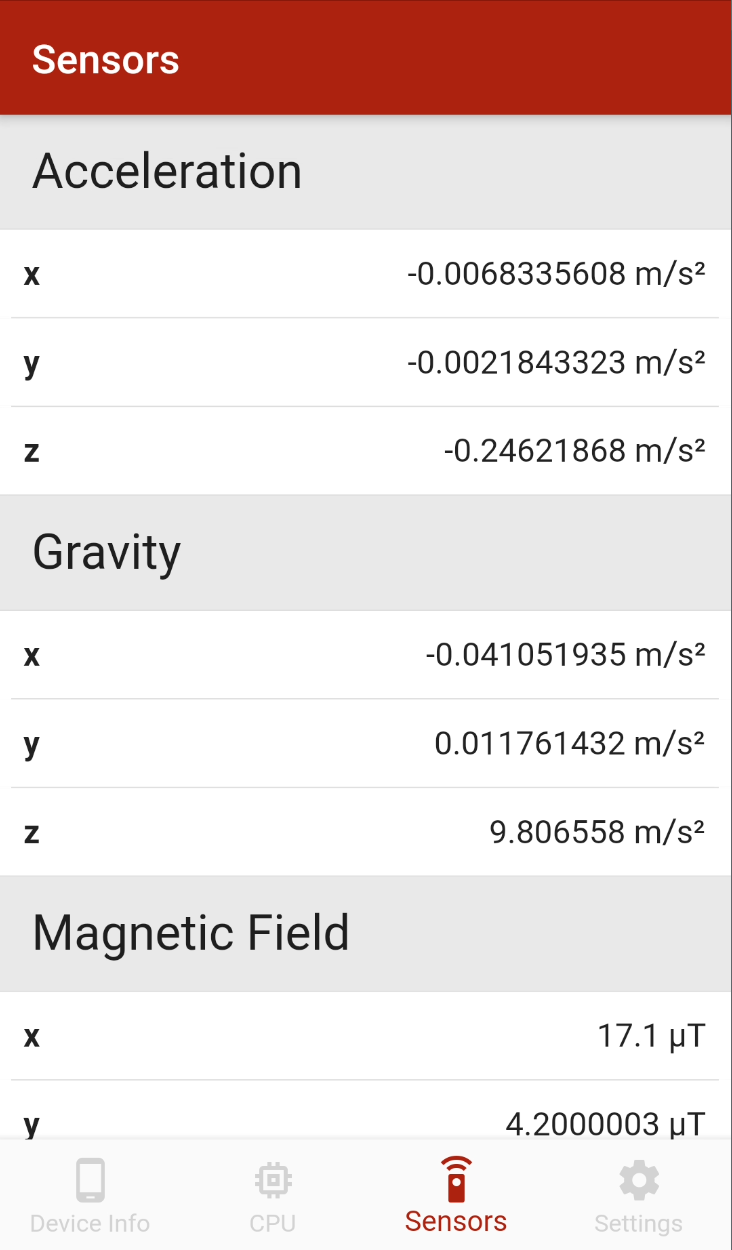
\includegraphics[height=20em]{mobile-sensors}
  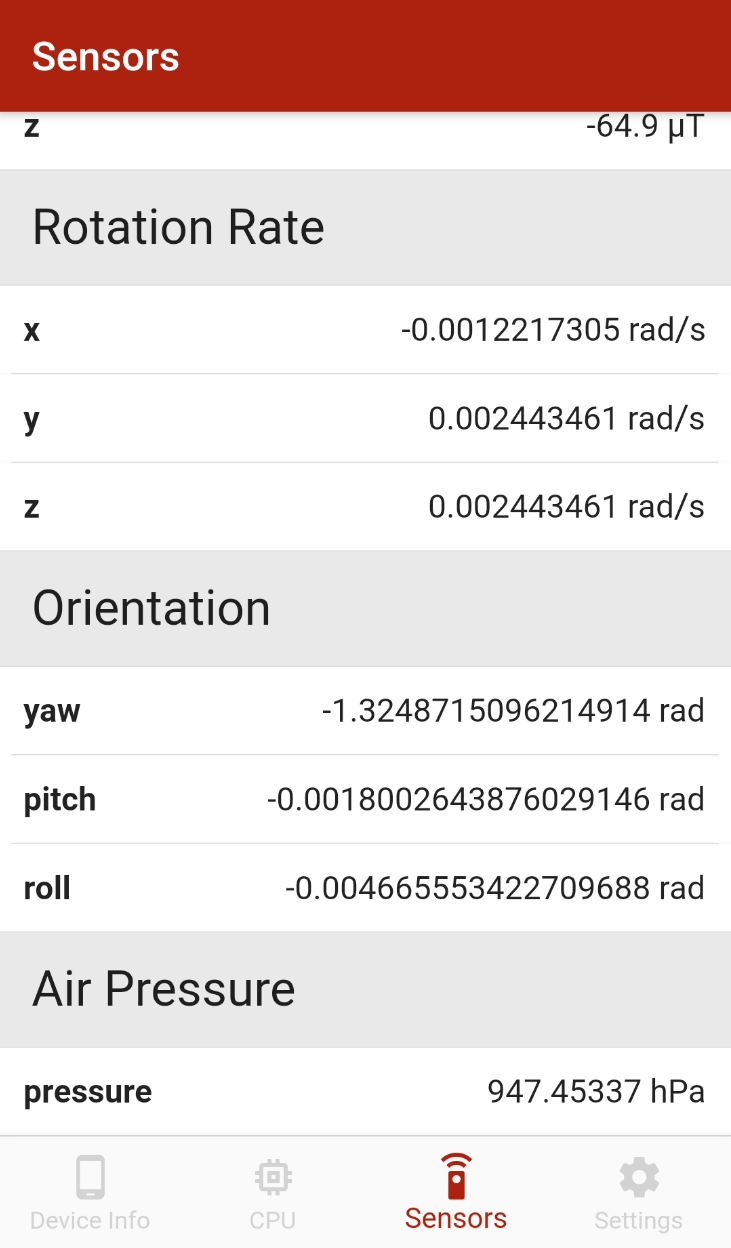
\includegraphics[height=20em]{mobile-sensors-2}
  \caption{\textit{Sensors} lists various sensors on both platforms.}
\end{figure}

\begin{figure}[H]
  \centering
  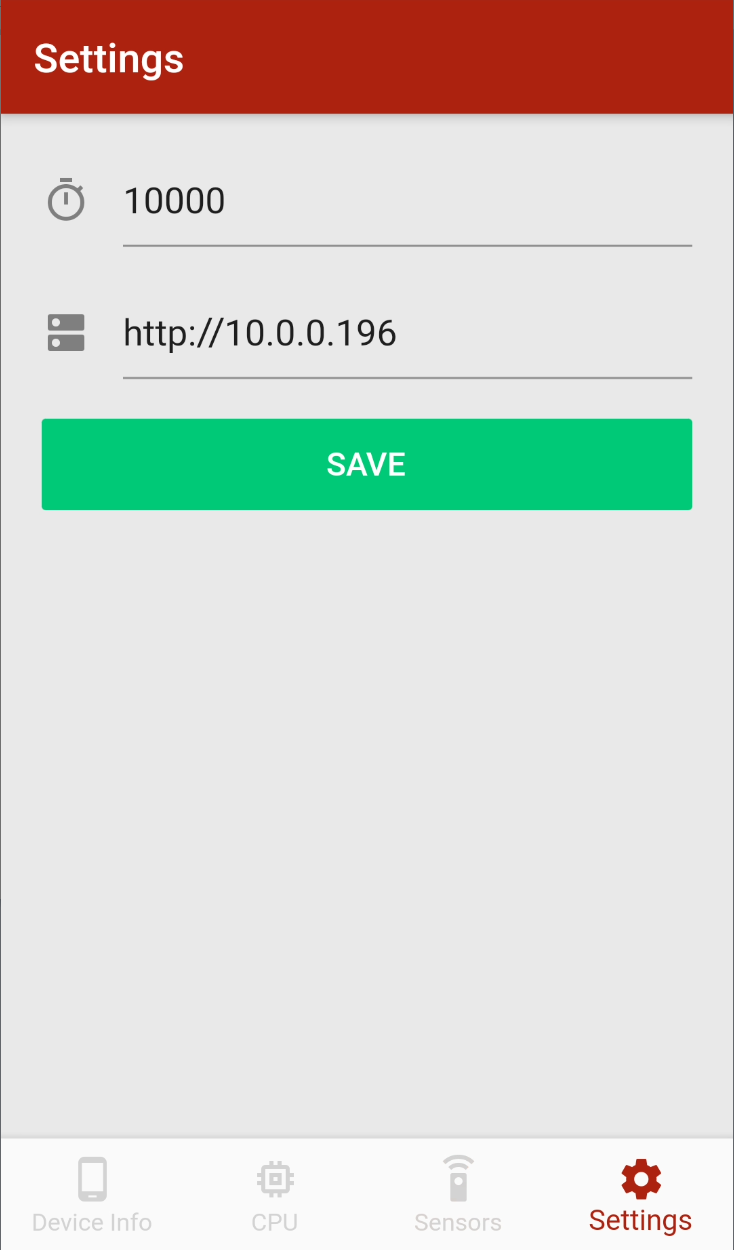
\includegraphics[height=20em]{mobile-settings}
  \caption{\textit{Settings} gives the user the ability to modify the interval of sending data to the
  server and the \textit{URL} where the server is located.}
\end{figure}

The most important part about the application however is sending data to a \textit{Kafka} topic
which then invokes a \textit{serverless function}. To achieve this we wrap all data into categories
and send them to the specific topic in \textit{Kafka} via \textit{JSON}. The task of the
\textit{serverless function} is then to push the data into our \textit{MongoDB} database.

\section{Serverless Stack}

Arguably, the main part of our thesis is the serverless stack hence it's also in the title of the
project. When doing research for our project, thinking about the serverless stack was one of the
first things we did. We came across many different serverless frameworks. \textit{OpenWhisk},
\textit{Fission} and \textit{Kubeless} just to name a few. While all of those seem to have their
benefits, none of them seemed to be as versatile as \textit{OpenFaaS}.

\textit{OpenFaaS} poses itself to have first class support for \textit{Docker Swarm} and being
\textit{Kubernetes} native. The former was particularly interesting for us as this meant that we
could test the framework without having to install any external tool except for  \textit{Docker}.

Running was as simple as cloning the \textit{OpenFaaS} repository, calling \texttt{docker swarm
init} and executing the provided initialisation script. Deploying an actual function is equally
simple. One has the option to either deploy a function from the store through the nicely designed
\textit{OpenFaaS} gateway on port~8080 or with the preferred way, which is using the
\texttt{faas-cli} command line tool.

Deploying a function from the store with it would look as follows:

\begin{lstlisting}[language=bash]
faas store deploy figlet
\end{lstlisting}

Here, \texttt{figlet} is the name of the function in the store.

After gaining a grasp of how the platform works, we decided to put our own spin on it by firstly
modifying the given deploy script to our needs and porting it from \textit{Bash} to \textit{Rust}
for it to be cross platform. The next step then was to write our own configuration file for swarm
deployment, namely \texttt{deploy.yml}. This \textit{YAML} file includes the configuration for
\textit{Kafka}, \textit{Zookeeper}, \textit{MongoDB}, various services that are needed for
\textit{OpenFaaS}, a bunch of gateways for visualisation and the \textit{Kafka-Connector}. All of
these service are \textit{Docker} images and can therefore be easily updated and extended.
\textit{Kafka-Connector} is particularly interesting, because its main purpose is to call a
serverless function on a Kafka topic change. To make a function react to a Kafka topic we can again
use our example store function \texttt{figlet}:

\begin{lstlisting}[language=bash]
faas store deploy figlet --annotation topic="faas-request"
\end{lstlisting}

The deployment aspect is the same as before, therefore the interesting part is the \\
\texttt{-{}-annotation} flag, where \texttt{topic="faas-request"} is the \textit{Kafka} topic the
function is supposed to listen to and act on. We subsequently can look for the result in the logs of
the connector service. \\
While the feature of deploying functions from the store is really nice, it is not suitable for our
use case, as we highly depend on custom functions written by ourselves.

\begin{figure}[H]
  \centering
  \adjincludegraphics[max width=\textwidth]{openfaas-dashboard}
  \caption{Picture of all functions in the \textit{OpenFaaS} dashboard}
\end{figure}

\section{Raspberry Pi}

In order for us to gather data, we decided on using multiple \textit{Raspberry Pis} with different
sensors attached to them. We chose the \textit{Raspberry Pi} because it is backed by a huge
community and because of the vast amount of documentation available for it. Having documentation
available was essential, since we wanted to write the client application for the \textit{Raspberry
Pi} in \textit{Rust}. This way we could validate our \textit{Rust} code by comparing it to example
code written in other programming languages, most commonly \textit{Python} or \textit{C} in the case
of the \textit{Raspberry Pi}.

\subsection{\textit{Rust} on the \textit{Raspberry Pi}}

For our first “Hello, world!” program which would run on the \textit{Raspberry Pi}, we took the
simplest approach at the time. We would write the code on our development machines and synchronise
the code to the \textit{Raspberry Pi} using \texttt{rsync} \cite{rsync} and then compile and run it
via \texttt{ssh}. This worked fine at the time. Once we got to the point where we needed to add more
dependencies for the various sensors and networking, compile times naturally increased to the point
at which it simply wasn't feasible anymore to compile directly using the inadequate processor of the
\textit{Raspberry Pi}. A single build was approaching a compile time of around five minutes on every
single small change to the code, so we had to start looking for alternatives.

\subsection{Cross Compilation}

Soon after we realised that compiling directly on the \textit{Raspberry Pi} was not a good solution,
we had to find a way to cross compile for the \textit{Raspberry Pi}. This was further complicated by
the fact the we were using \textit{macOS} and \textit{Windows}, so none of the pre-compiled cross
compilation \whitelist{toolchains} for \textit{Linux} were an option for us.

We then found the \texttt{cross} \cite{cross} tool, which claimed to automatically install the
corresponding toolchain and then run the cross compilation in a \textit{Docker} container, so this
should have worked on both \textit{macOS} and \textit{Windows}. Right after we installed it using
\texttt{cargo install cross}, we saw that \textit{macOS} and \textit{Windows} support was lacking.
On both platforms, \texttt{cross} tried to simply call \texttt{cargo} directly instead of running in
a \textit{Docker} container. Since this tool still seemed to be the best solution we could find for
our situation and since the tool is open-source, we decided to dig into the source code and add the
missing \textit{macOS} and \textit{Windows} support ourselves.

Getting \texttt{cross} to actually run a \textit{Docker} container on both of our platforms was
quite easy, we only had to add two new definitions for \textit{Rust} toolchains in the source code
of \texttt{cross}, one for \textit{macOS} (\texttt{x86\_64-apple-darwin}) and one for
\textit{Windows} (\texttt{x86\_64-pc-windows-msvc}). The next problem we were facing was that inside
of the \textit{Docker} container, the \texttt{CARGO\_HOME} directory was mounted, and with it, its
\texttt{bin} subdirectory. This meant that the \textit{Docker} container would first look in this
directory instead of the respective toolchain root for the corresponding target's binaries. Since
the binaries in \texttt{CARGO\_HOME/bin} are compiled for the host machine, these previously worked
fine since only \texttt{x86\_64} \textit{Linux} hosts were supported. Now however, it would try
running a \textit{macOS} or \textit{Windows} binary inside of a \textit{Linux} \textit{Docker}
container. This was not as straight-forward to debug as it might seem, since the error message made
it seem as though it was a syntax error in a shell command. Once we found what the problem was, the
next challenge was to actually implement the fix for it. We still had to mount \texttt{CARGO\_HOME},
but exclude its \texttt{bin} subdirectory. Since the contents of \texttt{CARGO\_HOME} can vary
depending on what you have installed, we could not simply mount each subdirectory individually and
exclude \texttt{bin}, so the only way was to use a somewhat hacky workaround.

The whole \texttt{CARGO\_HOME} directory was already mounted using

\begin{lstlisting}[language=Bash]
-v "${CARGO_HOME}:/cargo:Z"
\end{lstlisting}

In order to prevent mounting the \texttt{bin} subdirectory from the host machine, we added

\begin{lstlisting}[language=Bash]
-v /cargo/bin
\end{lstlisting}

This means that technically the \texttt{bin} subdirectory is still mounted, but is overlaid by
another virtual volume which is not bound to a directory on the host, which effectively prevents
non-Linux binaries from being accessible inside the \textit{Docker} container. After this change, we could
finally compile our program on both \textit{macOS} and \textit{Windows}.

\subsection{Sensors}

For the actual collection of data, we of course needed to implement some sensors. The first sensor
we implemented is the widely used \textit{BMP180}, a digital sensor which acts as a combination of a
thermometer and barometer. The \\ \textit{BMP180} communicates over the \textit{I\textsuperscript{2}C}
bus. \textit{I\textsuperscript{2}C} is supported natively by most \textit{Linux} distributions,
consequentially also by the \textit{Raspbian} operating system running on the \textit{Raspberry Pi}.
We quickly found a \textit{Rust} library called \texttt{i2cdev}, which provides idiomatic wrapper functions
to interface with the \textit{Linux} \textit{I\textsuperscript{2}C} interface. Another library
called \texttt{i2cdev\_bmp180} then gave us an API for performing temperature and air pressure
measurements.

The second sensor we wanted to implement is the \textit{AM2320}, a digital temperature and humidity
sensor. The \textit{AM2320} also communicates over the \textit{I\textsuperscript{2}C} bus, which
means we could use a \textit{Rust} library fittingly called \textit{am2320}, which also is based on the
\textit{i2cdev} library, to produce temperature and humidity measurements. We also contributed some
improvements (see \url{https://github.com/gferon/am2320.rs/pull/1}) to this library.

The last sensor we implemented is a simple analogue photoresistor acting as a luminosity sensor. Due
to the fact that the \textit{Raspberry Pi} does not have any analogue \textit{GPIO} pins, we had to
resort to using an analogue-to-digital converter. To simplify the implementation of such a
converter, we chose the \textit{ADS1115}, which like the \textit{BMP180} and \textit{AM2320}
communicates over the \textit{I\textsuperscript{2}C} bus. With the \texttt{ads1x1x} library, we
could read the analogue photoresistor's voltage. By knowing this voltage, we can then
approximate the luminosity.

\begin{figure}[H]
  \centering
  \adjincludegraphics[max width=\textwidth]{wiring}
  \caption{Wiring diagram of sensors connected to a \textit{Raspberry Pi}}
  \label{fig:raspberry-wiring}
\end{figure}

In \autoref{fig:raspberry-wiring} we can see how the sensors are connected to the \textit{Raspberry
Pi}. The orange and red wires signify the 3.3V and 5V power supply lanes, respectively. The black
wire is the ground connection, and blue and violet are the two wires (receive/transmit) for the
\textit{I\textsuperscript{2}C} bus. From top to bottom, you can see the photoresistor connected to
the analogue-to-digital converter (ADC), followed by the \textit{BMP180} and the \textit{AM2320}. It
is easy to see that all sensors share the same \textit{I\textsuperscript{2}C} bus by looking at the
diagram.

\subsection{Serverless UI}

Another instrumental part of the project is the UI. Without any form of visualisation our whole data
gathering process would not be of much use. For this reason we decided early on what kind of front
end web development stack we would use. Since both us are familiar with \textit{React} - a
\textit{JavaScript} framework famous for revolutionising the use of the \textit{virtual DOM}
to render \textit{UI} elements and to update \textit{UI} elements reactively on
UI change - we decided on using \textit{MarkoJS}.

\subsubsection{MarkoJS}

\textit{MarkoJS} shares many of the same benefits as \textit{React} with some added flexibility like
\textit{concise HTML syntax} which makes the whole \textit{markup} more readable and easier to
write. It also has the ability to use conventional control flow structures like \textit{if} or
\textit{for} directly in the \textit{markup}.

\subsubsection{Babel}

However \textit{MarkoJS} is most and foremost a \textit{JavaScript} framework and due to the nature
of the before mentioned features, \textit{transpiling} is inevitable. \textit{Transpiling} means to
transform modern possibly unsupported \textit{JavaScript} into valid \textit{ECMAScript 5} compliant
code that any browser can understand. For this process we currently use the industry standard
technology \textit{Babel}. With \textit{Babel} \textit{transpiling} is rather easy. All necessary
definitions are in a \textit{webpack.config.babel.js} file which brings us to the next essential
tool \textit{Webpack}.

\subsubsection{Webpack}

“Webpack is a module bundler. Its main purpose is to bundle JavaScript files for usage in a browser,
yet it is also capable of transforming, bundling, or packaging just about any resource or asset.”

With that being said \textit{Webpack} can to some extend be considered as the main part of the whole
\textit{front end stack} as it is responsible for orchestrating \textit{transpiling} of
\textit{MarkoJS} files. It is also responsible for providing \textit{Webpack Dev Server}, a server
that reloads on file change. Furthermore \textit{Webpack} runs all files through certain
optimisation plugins on release build, which can bring down the size of the \textit{code bundle}
quite considerably. \textit{Webpack} is also able to transform \textit{SASS} into \textit{CSS}.

\subsubsection{SASS}

\textit{SASS} is a superset of \textit{CSS} with many additional features like variables, functions,
nesting and exporting / importing files. We make heavy use of those features to structure and
modularise our \textit{CSS} code.

\subsection{UI}

The \textit{UI} itself uses a basic layout where all sensor devices registered in the database are
listed on the side in a so called \textit{sidebar}. The user then can click on each individual
device to open a view with detailed graphs of sensor data of that device. The categories of graphs
are different according to device group. For example \textit{IoT devices} will have different
sensors compared to phones. After a device is selected, the user can then specify the begin and end
time interval according to which sensor data of that device will be filtered and the amount of time
slices. By default the timespan is limited to 24 hours and to 24 time slices. A time slice in our
case is a division of a time interval into equally long time units. To get a single value per time
slice we average all sensor values of a specific sensor between two time slices. Those single values
will then be displayed in the graphs.

\subsection{Azure Pipelines}

In order to properly verify our results we used \textit{Azure Pipelines} as our continues integration service
of choice. \textit{Azure Pipelines} offers 10 parallel jobs with unlimited time per job for
open source projects. \cite{azure-pipelines-devop}

In our case we used the \textit{CI} platform for 6 jobs, that are \textit{app}, \textit{rpi}
\textit{functions}, \textit{ui} and \textit{tex}.

In \textit{app} we build and test our \textit{Flutter mobile application}. For the \textit{vmImage}
the job will run on we have to choose \textit{macOS} in order to build the application for
\textit{Android} and \textit{iOS} since \textit{Apple} restricts building of \textit{iOS apps} to
\textit{macOS}.

The \textit{rpi} job is responsible for building and testing the application, that will be deployed
on the \textit{Rasperry Pi} in order to measure sensor data. The program is written in
\textit{Rust}. Because \textit{Rust} is cross platform, a conventional \textit{Ubuntu} image is
sufficient. Unfortunately \textit{Azure Pipelines} virtual machines do not have \textit{Rust}
installed by default, therefore we have to rely on a template provided by the \textit{Rust Cargo
team} \cite{rust-cargo}. This \textit{Azure Pipelines} job however is not trivial and requires
multiple steps. \textit{Rasperry Pis} use \textit{ARM} as there instruction set and therefore differ
from the instruction set used in the virtual machines of \textit{Azure}. A simple compile of the
application is for this reason not possible. In order to run the program on the \textit{Rasperry
PI}, the application actually has to be cross compiled with the correct toolchain
\textit{armv7-unknown-linux-gnueabi}.

